%\documentclass[hyperref={pdfpagelabels=false},slidetop,9pt]{beamer}
\documentclass[slidetop,8pt]{beamer}
\usepackage[T1]{fontenc}
\usepackage[utf8]{inputenc}
\newcommand{\id}{71}
\newcommand{\nom}{Théorie des mécanismes}
\newcommand{\sequence}{04}
\newcommand{\nomsequence}{Liaisons entre les solides}
\newcommand{\num}{02}
\newcommand{\type}{KH}
\newcommand{\descrip}{Liaisons équivalentes, hyperstatisme, liaisons en série et en parallèle, théorie des graphes}
\newcommand{\competences}{B2-12: Proposer une modélisation des liaisons avec leurs caractéristiques géométriques. \\ &  B2-13: Proposer un modèle cinématique paramétré à partir d'un système réel, d'une maquette numérique ou d'u \\ &  B2-17: Simplifier un modèle de mécanisme. \\ &  B2-18: Modifier un modèle pour le rendre isostatique. \\ &  C1-04: Proposer une démarche permettant d'obtenir une loi entrée-sortie géométrique.  \\ &  C2-05: Caractériser le mouvement d'un repère par rapport à un autre repère. \\ &  C2-06: Déterminer les relations entre les grandeurs géométriques ou cinématiques. }
\newcommand{\nbcomp}{7}
\newcommand{\systemes}{}
\newcommand{\systemesnum}{}
\newcommand{\systemessansaccent}{}
\newcommand{\ilot}{2}
\newcommand{\ilotstr}{02}
\newcommand{\dossierilot}{\detokenize{Ilot_02 }}

\usepackage{etex}
\usepackage{tikz}
\usepackage[european]{circuitikz}
\usepackage{pgf}
\usepackage[all]{xy}
\usepackage{pgfpages}
\usepackage{graphbox}
\usepackage{pdfpages}
%\usepackage[adobe-utopia]{mathdesign}
\usepackage{ifthen}
\usepackage{cancel}
\usepackage{framed}
\usepackage{subfig}
\usepackage{tabularx}
\usepackage{setspace}
\usepackage{soul}
\usepackage{schemabloc}
\usepackage{eqnarray}
\usepackage[dot, phantomtext]{dashundergaps}
\usepackage{media9}
\usepackage{multimedia}
\usepackage{textcomp}
\usefonttheme[onlymath]{serif}

\author{Renaud Costadoat}
\institute{Lycée Dorian}

\usepackage{multido}
\usepackage{multirow}
\usepackage{multicol} % Portions de texte en colonnes
\usepackage{flafter}%floatants après la référence

\usepackage{color}
\usepackage{xcolor}
\usepackage{colortbl}

\usepackage[gen]{eurosym}
\usepackage{tikz}
%\usepackage{pstricks,pst-node,pst-tree,pst-solides3d}
\usepackage{lmodern}
\usepackage[francais]{babel}
\usepackage{pslatex}
\usetheme{renaud}
\usepackage{times}
\usepackage[frenchmath]{newtxsf} % for sans serif symbols
\renewcommand{\familydefault}{\sfdefault}
%\usepackage{amsfonts}
%\usepackage{amsmath}
%\usepackage{mathastext}
\usepackage{verbatim}
\usepackage{moreverb}
%\usetikzlibrary{arrows,shapes}
\usepackage{graphicx}
\usepackage{psfrag}
\usepackage{wrapfig}
\usepackage{etoolbox}

\definecolor{gris25}{gray}{0.75}
\definecolor{bleu}{RGB}{18,33,98}
\definecolor{bleuf}{RGB}{42,94,171}
\definecolor{bleuc}{RGB}{231,239,247}
\definecolor{rougef}{RGB}{185,18,27}
\definecolor{rougec}{RGB}{255,188,204}%255,230,231
\definecolor{vertf}{RGB}{103,126,82}
\definecolor{vertc}{RGB}{220,255,191}

\setlength\parindent{24pt}
\parskip 7.2pt
\parindent 8pt

\newenvironment{rem}[1][\hsize]%
{%
    \def\FrameCommand
   {%
\rotatebox{90}{\textit{\textsf{Remarque}}} 
       {\color{bleuf}\vrule width 3pt}%
       \hspace{0pt}%must no space.
       \fboxsep=\FrameSep\colorbox{bleuc}%
  }%
    \MakeFramed{\hsize#1\advance\hsize-\width\FrameRestore}%
}%
{\endMakeFramed}%


\newenvironment{savoir}[1][\hsize]%
{%
    \def\FrameCommand
    {%
\rotatebox{90}{\textit{\textsf{Savoir}}} 
        {\color{bleuf}\vrule width 3pt}%
        \hspace{0pt}%must no space.
        \fboxsep=\FrameSep\colorbox{bleuc}%
    }%
    \MakeFramed{\hsize#1\advance\hsize-\width\FrameRestore}%
}%
{\endMakeFramed}%

\newenvironment{prob}[1][\hsize]%
{%
    \def\FrameCommand%
    {%
\rotatebox{90}{\textit{\textsf{Problematique}}} 
        {\color{rougef}\vrule width 3pt}%
        \hspace{0pt}%must no space.
        \fboxsep=\FrameSep\colorbox{rougec}%
    }%
    \MakeFramed{\hsize#1\advance\hsize-\width\FrameRestore}%
}%
{\endMakeFramed}%

\newenvironment{obj}[1][\hsize]%
{%
    \def\FrameCommand%
    {%
\rotatebox{90}{\textit{\textsf{Objectif}}} 
        {\color{vertf}\vrule width 3pt}%
        \hspace{0pt}%must no space.
        \fboxsep=\FrameSep\colorbox{vertc}%
    }%
    \MakeFramed{\hsize#1\advance\hsize-\width\FrameRestore}%
}%
{\endMakeFramed}%

\newenvironment{defi}[1][\hsize]%
{%
    \def\FrameCommand%
    {%
\rotatebox{90}{\textit{\textsf{Definition}}} 
        {\color{bleuf}\vrule width 3pt}%
        \hspace{0pt}%must no space.
        \fboxsep=\FrameSep\colorbox{rougec}%
    }%
    \MakeFramed{\hsize#1\advance\hsize-\width\FrameRestore}%
}%
{\endMakeFramed}%


\newenvironment{hypo}[1][\hsize]%
{%
    \def\FrameCommand%
    {%
\rotatebox{90}{\textit{\textsf{Hypothèse\\}}} 
        {\color{bleuf}\vrule width 3pt}%
        \hspace{0pt}%must no space.
        \fboxsep=\FrameSep\colorbox{bleuc}%
    }%
    \MakeFramed{\hsize#1\advance\hsize-\width\FrameRestore}%
}%
{\endMakeFramed}%


\newenvironment{prop}[1][\hsize]%
{%
    \def\FrameCommand%
    {%
\rotatebox{90}{\textit{\textsf{Propriété}}} 
        {\color{bleuf}\vrule width 3pt}%
        \hspace{0pt}%must no space.
        \fboxsep=\FrameSep\colorbox{bleuc}%
    }%
    \MakeFramed{\hsize#1\advance\hsize-\width\FrameRestore}%
}%
{\endMakeFramed}%

\newenvironment{props}[1][\hsize]%
{%
    \def\FrameCommand%
    {%
\rotatebox{90}{\textit{\textsf{Propriétés}}} 
        {\color{bleuf}\vrule width 3pt}%
        \hspace{0pt}%must no space.
        \fboxsep=\FrameSep\colorbox{bleuc}%
    }%
    \MakeFramed{\hsize#1\advance\hsize-\width\FrameRestore}%
}%
{\endMakeFramed}%

\newenvironment{exemple}[1][\hsize]%
{%
    \def\FrameCommand%
    {%
\rotatebox{90}{\textit{\textsf{Exemple}}} 
        {\color{vertf}\vrule width 3pt}%
        \hspace{0pt}%must no space.
        \fboxsep=\FrameSep\colorbox{vertc}%
    }%
    \MakeFramed{\hsize#1\advance\hsize-\width\FrameRestore}%
}%
{\endMakeFramed}%

\newenvironment{resultat}[1][\hsize]%
{%
    \def\FrameCommand%
    {%
\rotatebox{90}{\textit{\textsf{Résultat}}} 
        {\color{rougef}\vrule width 3pt}%
%        {\color{bleuf}\vrule width 3pt}%
        \hspace{0pt}%must no space.
        \fboxsep=\FrameSep\colorbox{rougec}%
    }%
    \MakeFramed{\hsize#1\advance\hsize-\width\FrameRestore}%
}%
{\endMakeFramed}%

\newenvironment{methode}[1][\hsize]%
{%
    \def\FrameCommand%
    {%
\rotatebox{90}{\textit{\textsf{Méthode\\}}} 
        {\color{rougef}\vrule width 3pt}%
        \hspace{0pt}%must no space.
        \fboxsep=\FrameSep\colorbox{rougec}%
    }%
    \MakeFramed{\hsize#1\advance\hsize-\width\FrameRestore}%
}%
{\endMakeFramed}%

\newenvironment{theo}[1][\hsize]%
{%
    \def\FrameCommand%
    {%
\rotatebox{90}{\textit{\textsf{Théorème\\}}} 
        {\color{rougef}\vrule width 3pt}%
        \hspace{0pt}%must no space.
        \fboxsep=\FrameSep\colorbox{rougec}%
    }%
    \MakeFramed{\hsize#1\advance\hsize-\width\FrameRestore}%
}%
{\endMakeFramed}%

\newenvironment{warn}[1][\hsize]%
{%
    \def\FrameCommand%
    {%
\rotatebox{90}{\textit{\textsf{Attention\\}}} 
        {\color{rougef}\vrule width 3pt}%
        \hspace{0pt}%must no space.
        \fboxsep=\FrameSep\colorbox{rougec}%
    }%
    \MakeFramed{\hsize#1\advance\hsize-\width\FrameRestore}%
}%
{\endMakeFramed}%

% \usepackage{pstricks}
%\usepackage{minitoc}
% \setcounter{minitocdepth}{4}

\setcounter{tocdepth}{2}

% \mtcselectlanguage{french} 

%\usepackage{draftcopy}% "Brouillon"
% \usepackage{floatflt}
\usepackage{psfrag}
%\usepackage{listings} % Permet d'insérer du code de programmation
\renewcommand{\baselinestretch}{1.2}

% Changer la num�rotation des figures :
% ------------------------------------
% \makeatletter
% \renewcommand{\thefigure}{\ifnum \c@section>\z@ \thesection.\fi
%  \@arabic\c@figure}
% \@addtoreset{figure}{section}
% \makeatother
 


%%%%%%%%%%%%
% Définition des vecteurs %
%%%%%%%%%%%%
 \newcommand{\vect}[1]{\overrightarrow{#1}}

%%%%%%%%%%%%
% Définition des torseusr %
%%%%%%%%%%%%

 \newcommand{\torseur}[1]{%
\left\{{#1}\right\}
}

\newcommand{\torseurcin}[3]{%
\left\{\mathcal{#1} \left(#2/#3 \right) \right\}
}

\newcommand{\torseurstat}[3]{%
\left\{\mathcal{#1} \left(#2\rightarrow #3 \right) \right\}
}

 \newcommand{\torseurc}[8]{%
%\left\{#1 \right\}=
\left\{
{#1}
\right\}
 = 
\left\{%
\begin{array}{cc}%
{#2} & {#5}\\%
{#3} & {#6}\\%
{#4} & {#7}\\%
\end{array}%
\right\}_{#8}%
}

 \newcommand{\torseurcol}[7]{
\left\{%
\begin{array}{cc}%
{#1} & {#4}\\%
{#2} & {#5}\\%
{#3} & {#6}\\%
\end{array}%
\right\}_{#7}%
}

 \newcommand{\torseurl}[3]{%
%\left\{\mathcal{#1}\right\}_{#2}=%
\left\{%
\begin{array}{l}%
{#1} \\%
{#2} %
\end{array}%
\right\}_{#3}%
}

 \newcommand{\vectv}[3]{%
\vect{V\left( {#1} \in {#2}/{#3}\right)}
}


\newcommand{\vectf}[2]{%
\vect{R\left( {#1} \rightarrow {#2}\right)}
}

\newcommand{\vectm}[3]{%
\vect{\mathcal{M}\left( {#1}, {#2} \rightarrow {#3}\right)}
}


 \newcommand{\vectg}[3]{%
\vect{\Gamma \left( {#1} \in {#2}/{#3}\right)}
}

 \newcommand{\vecto}[2]{%
\vect{\Omega\left( {#1}/{#2}\right)}
}

\newcommand{\reponse}[1][4]
{
\multido{}{#1}
{
\begin{center}
\makebox[0.9\linewidth]{\dotfill} \end{center}
}}


% }$$\left\{\mathcal{#1} \right\}_{#2} =%
% \left\{%
% \begin{array}{c}%
%  #3 \\%
%  #4 %
% \end{array}%
% \right\}_{#5}}


%  ------------------------------------------
% | Modification du formatage des sections : | 
%  ------------------------------------------

% Grands titres :
% ---------------

\newcommand{\titre}[1]{%
\begin{center}
      \bigskip
      \rule{\textwidth}{1pt}
      \par\vspace{0.1cm}
      
      \textbf{\large #1}
      \par\rule{\textwidth}{1pt}
    \end{center}
    \bigskip
  }

% Supprime le numéro du chapitre dans la numérotation des sections:
% -----------------------------------------------------------------
\makeatletter
\renewcommand{\thesection}{\@arabic\c@section}
\makeatother


% \titleformat{\chapter}[display]
% {\normalfont\Large\filcenter}
% {}
% {1pc}
% {\titlerule[1pt]
%   \vspace{1pc}%
%   \Huge}[\vspace{1ex}%
% \titlerule]


%%%% Chapitres Comme PY Pechard %%%%%%%%%
% numéro du chapitre
\DeclareFixedFont{\chapnumfont}{OT1}{phv}{b}{n}{80pt}
% pour le mot " Chapitre "
\DeclareFixedFont{\chapchapfont}{OT1}{phv}{m}{it}{40pt}
% pour le titre
\DeclareFixedFont{\chaptitfont}{T1}{phv}{b}{n}{25pt}

\definecolor{gris}{gray}{0.75}
\setbeamertemplate{section in toc}[sections numbered]

\newlength{\RoundedBoxWidth}
\newsavebox{\GrayRoundedBox}
\newenvironment{GrayBox}[1][\dimexpr\textwidth-4.5ex]%
   {\setlength{\RoundedBoxWidth}{\dimexpr#1}
    \begin{lrbox}{\GrayRoundedBox}
       \begin{minipage}{\RoundedBoxWidth}}%
   {   \end{minipage}
    \end{lrbox}
    \begin{center}
    \begin{tikzpicture}%
       \draw node[draw=bleuf,fill=bleuc,rounded corners,%
             inner sep=2ex,text width=\RoundedBoxWidth]%
             {\usebox{\GrayRoundedBox}};
    \end{tikzpicture}
    \end{center}}
    
\ifdef{\prive}{\pgfpagesuselayout{2 on 1}[a4paper,border shrink=0mm]}
\ifdef{\prive}{\setbeamertemplate{navigation symbols}{}}
\setbeamertemplate{itemize item}[ball]
%\setbeamertemplate{blocks}[rounded]%[shadow=true]
\setbeamercolor{block title}{fg=white,bg=grisf}        % titre block normal 
\setbeamercolor{block body}{fg=grisf,bg=grisc!50}      % corps block normal
\setbeamercolor{block body alerted}{fg=white,bg=warning}   % idem pour un block alerte

\title{\nom}
\date{S\sequence \ - \type\num}

\begin{document}
\shorthandoff{:!}
\bibliographystyle{abbrvnat-fr}

\usebackgroundtemplate%
{%
    \centering
\includegraphics[width=\paperwidth]{/home/renaud/Documents/Renaud/GitHub/Sciences-Ingenieur/img/fond2}%
}

{
\setbeamertemplate{navigation symbols}{}
\setbeamertemplate{headline}[pagetitre]
\setbeamertemplate{footline}[pagetitre]
\usebackgroundtemplate{\centering
\includegraphics[width=\paperwidth]{/home/renaud/Documents/Renaud/GitHub/Sciences-Ingenieur/img/fond}}
\frame{\titlepage}
}



\section{Production}

\ifdef{\prive}{}{
\begin{frame}
\frametitle{Table des matières}
\tableofcontents[currentsection]
\end{frame}}
 
{\frame{
\frametitle{Production d'énergie en France}

\begin{minipage}{0.3\linewidth}
\begin{itemize}
 \item 1524TWh en 2021,
 \item 3/4 de nucléaire,
 \item pas de production d'hydrocarbures,
 \item statut particulier du nucléaire,
 \item baisse de la production.
\end{itemize}
\end{minipage}
\hfill
\begin{minipage}{0.65\linewidth}
\begin{figure}
    \centering
    \def\svgwidth{\linewidth}
    \input{img/figure-2-1-1-prod-primaire-CGDD.pdf_tex}
\end{figure}
\end{minipage}

Causes de la baisse de production:
\vspace{-0.5cm}
\begin{itemize}
 \item éolien en baisse (climat),
 \item hydraulique en baisse car les stocks en 2021 étaient plus faibles qu'en 2020,
 \item photovoltaïque (+12,6\%) mais sa place est faible (14\% photovoltaïque, 53\% hydraulique, 33\% éolien).
 \item production thermique grâce aux déchets (+10,4\%), risque de culture exclusive (betterave).
\end{itemize}
}}

{\frame{
\frametitle{Transformation d'énergie en France}

La transformation d'énergie consiste à transformer une source d'énergie en 
une autre énergie.

C'est une activité très faible en France:
\begin{itemize}
 \item Les centrales aux gaz n'ont quasiment pas été utilisées en 2021 à cause du prix,
 \item Il n'y a presque plus de raffineries en France,
 \item Les centrales à biogaz et biomasse ont augmenté par rapport à 2020.
\end{itemize}
}}

\section{Importation}

\ifdef{\prive}{}{
\begin{frame}
\frametitle{Table des matières}
\tableofcontents[currentsection]
\end{frame}}

{\frame{
\frametitle{Importation d'énergie en France}
Bilan énergétique de la France par type d'énergie en 2021 en millions de tonne d'équivalent pétrole.

\begin{table}
\resizebox{\textwidth}{!}{%
\begin{tabular}{|c|c|c|c|c|c|c|c|c|c|}
\hline
&Charbon&Pétrole&Gaz&Nucléaire&EnR&EnR&Électricité&Chaleur&Ensemble\\
&&&&&électriques&thermiques&&vendue&\\
&&&&&&et déchets&&&\\
\hline
Approvisionnement&&&&&&&&&\\
\hline
Production d'énergie primaire&0,0&0,8&0,0&98,8&9,6&21,8&0,0&///&131,0\\
\hline
Importations&6,0&81,3&40,7&0,0&0,0&2,1&1,8&///&132,0\\
\hline
Exportations&0,0&-13,3&-5,1&0,0&0,0&-0,7&-5,5&///&-24,7\\
\hline
Variation de stocks&1,2&1,0&1,4&0,0&0,0&0,0&0,0&///&3,6\\
\hline
Soutes maritimes et aériennes
internationales&0,0&-3,8&0,0&0,0&0,0&0,0&0,0&///&-3,8\\
\hline
Total des disponibilités&7,2&66,0&37,0&98,8&9,6&23,1&-3,6&///&238,1\\
\hline
Taux d'indépendance énergétique (en \%)&///&1,2&///&100,0&100,0&94,1&///&///&55,0\\
\hline
Emplois&&&&&&&&&\\
\hline
Consommation de la branche énergie&6,0&2,1&7,0&98,8&9,6&6,5&-41,0&-3,9&85,1\\
\hline
Consommation finale énergétique&0,9&52,2&28,9&0,0&0,0&16,6&37,3&3,9&139,9\\
\hline
Agriculture, industrie (y c. construction)&0,8&6,0&10,1&0,0&0,0&2,3&10,4&1,6&31,3\\
\hline
Résidentiel, tertiaire&0,1&7,0&18,5&0,0&0,0&11,4&26,1&2,3&65,5\\
\hline
Transports&0,0&39,2&0,3&0,0&0,0&2,8&0,8&0,0&43,1\\
\hline
Consommation finale non énergétique&0,3&11,7&1,1&0,0&0,0&0,0&0,0&0,0&13,0\\
\hline
Consommation totale d'énergie primaire&7,2&66,0&37,0&98,8&9,6&23,1&-3,6&0,0&238,1\\
\hline
\end{tabular}}
\end{table}

Source : SDES.

}}

{\frame{
\frametitle{Importation d'énergie en France}

\begin{center}
\begin{minipage}{0.7\linewidth}
\begin{defi}
$\text{Taux d'indépendance}=\dfrac{\text{Production primaire}}{\text{Consomation primaire}}=55\%$
\end{defi}
\end{minipage}
\end{center}
\vspace{-0.2cm}

Exemple, répartition des origines d'importation de gaz naturel:\vspace{-0.2cm}
\begin{figure}
    \centering
    \def\svgwidth{0.8\linewidth}
    \input{img/importation-gaz-naturel-CGDD.pdf_tex}
\end{figure}

}}

{\frame{
\frametitle{Facture énergétique de la France}

La facture s'élève à 44,3 milliards d'Euro en 2021.

Facture énergétique par type d'énergie:
\vspace{-0.2cm}
\begin{figure}
    \centering
    \def\svgwidth{0.8\linewidth}
    \input{img/facture-energetique-type-CGDD.pdf_tex}
\end{figure}

}}

\section{Consommation}

\ifdef{\prive}{}{
\begin{frame}
\frametitle{Table des matières}
\tableofcontents[currentsection]
\end{frame}}

{\frame{
\frametitle{Consommation énergétique de la France}

2769TWh ont été consommé en 2021:
\begin{itemize}
 \item 1778TWh en consommation finale,
 \item le reste en pertes et transports (c'est du majoritairement à la non récupération de l'eau chaude dans les centrales nucléaires).
\end{itemize}

Répartition:
\begin{itemize}
 \item 44\% pour les bâtiments tertiaires et résidence,
 \item 22\% pour l'agriculture et l'industrie,
 \item 31\% pour le transport.
\end{itemize}

}}

{\frame{
\frametitle{Consommation énergétique de la France}

\begin{figure}
    \centering
    \def\svgwidth{0.8\linewidth}
    \input{img/repartition-conso-energ-primaire-CGDD.pdf_tex}
\end{figure}

}}

{\frame{
\frametitle{Consommation énergétique de la France}

\begin{figure}
    \centering
    \def\svgwidth{0.8\linewidth}
    \input{img/ensemble-des-energies-CGDD.pdf_tex}
\end{figure}
}}

\section[PPE]{Programmations pluriannuelles de l’énergie}

\ifdef{\prive}{}{
\begin{frame}
\frametitle{Table des matières}
\tableofcontents[currentsection]
\end{frame}}

{\frame{
\frametitle{Le rapport du GIEC}

\begin{minipage}{0.42\linewidth}

\textbf{GIEC (Groupe d'experts intergouvernemental sur l'évolution du climat)}

Démonstration des effets du changement climatique sur l'ensemble des régions du globe:\begin{itemize}
 \item vagues de chaleur,
 \item perturbation des précipitations,
 \item sécheresses plus fréquentes et plus intenses,
 \item montée du niveau des océans,
 \item risque accru de submersion marine, etc...
\end{itemize}

Intensification des changements à mesure que le réchauffement global va continuer: seuil de +1,1°C déjà franchi.


\end{minipage}
\hfill
\begin{minipage}{0.5\linewidth}
\begin{figure}
	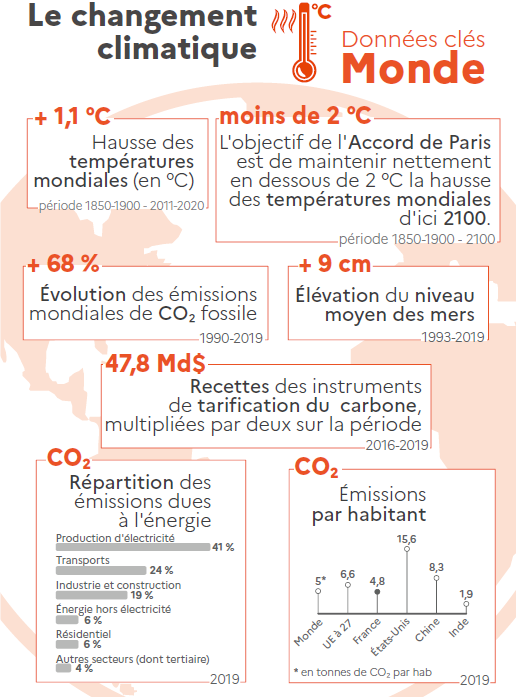
\includegraphics[width=1\linewidth]{img/chiffres_cles_climat_mondeedition2022.v2_0.png}
\end{figure}
\end{minipage}
}}

{\frame{
\frametitle{Conséquences du réchauffement climatique}
\begin{figure}
	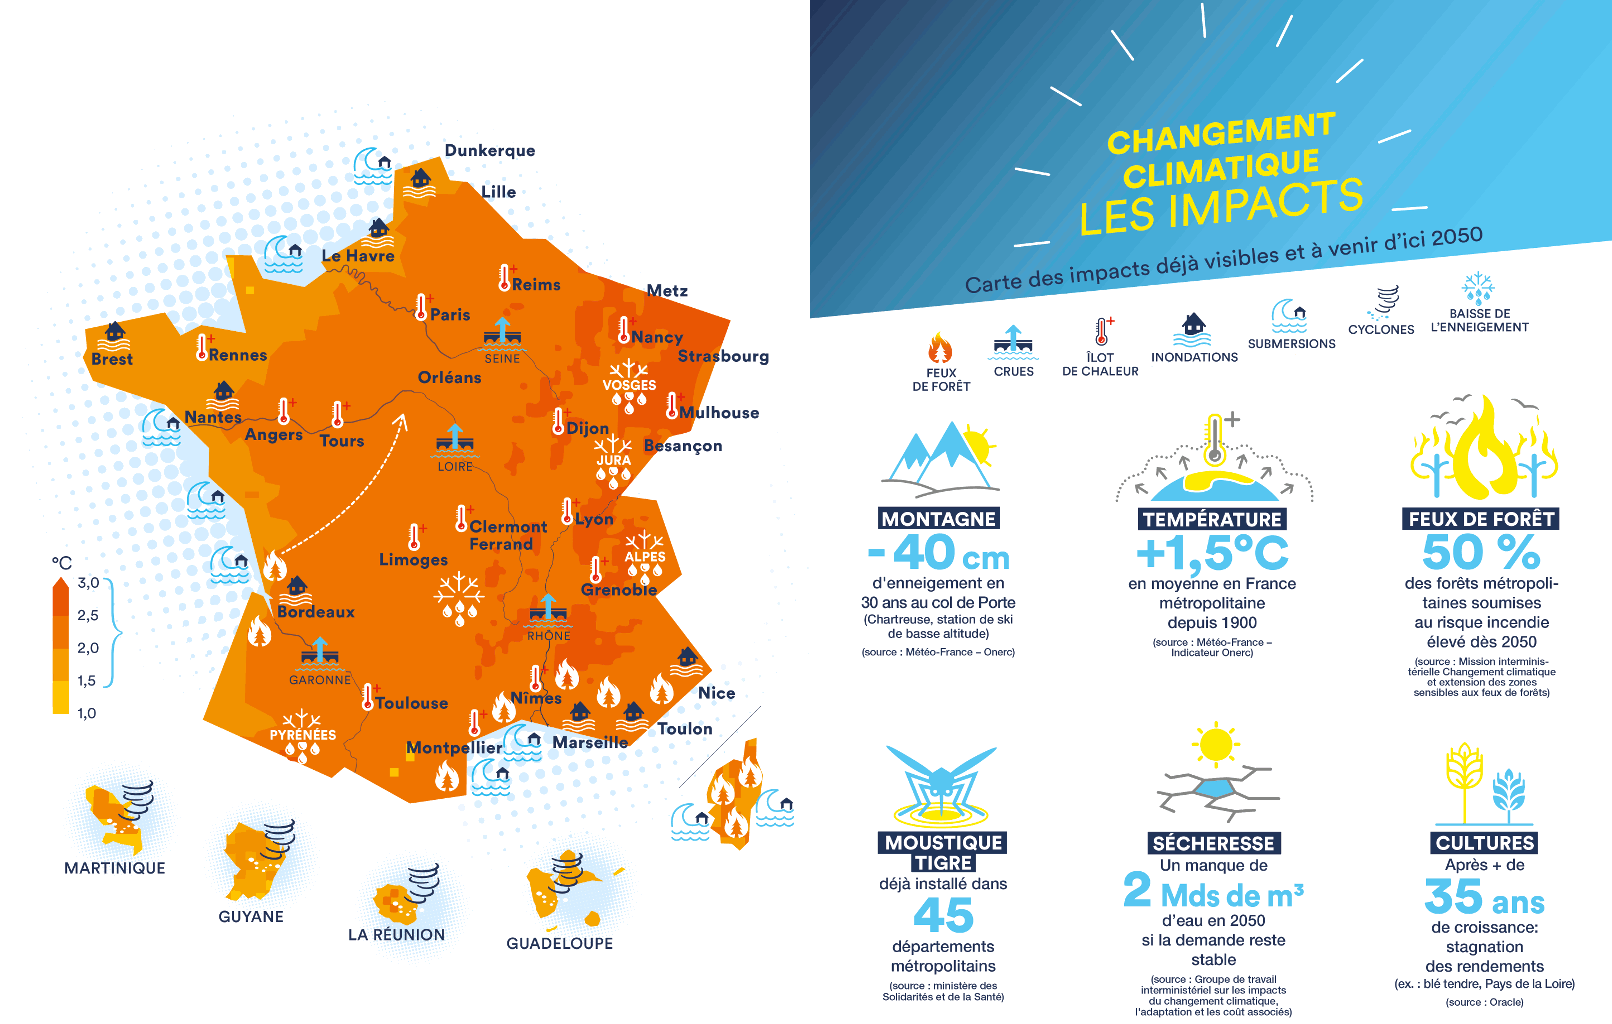
\includegraphics[width=1\linewidth]{img/18140_pnacc2_infog_v3-810.png}
\end{figure}
}}

{\frame{
\frametitle{Conséquences du réchauffement climatique}

\begin{minipage}{0.4\linewidth}

A cela s'ajoute:
\begin{itemize}
 \item disparition de la faune et de la flore,
 \item conflit armés,
 \item famines,
 \item maladies,
 \item réfugiés climatiques,
 \item risque de fonte du permafrost (réserve de méthane).
\end{itemize}

\end{minipage}
\hfill
\begin{minipage}{0.5\linewidth}
    \begin{figure}
    \begin{tikzpicture}
    \node at (-0.5,-3) {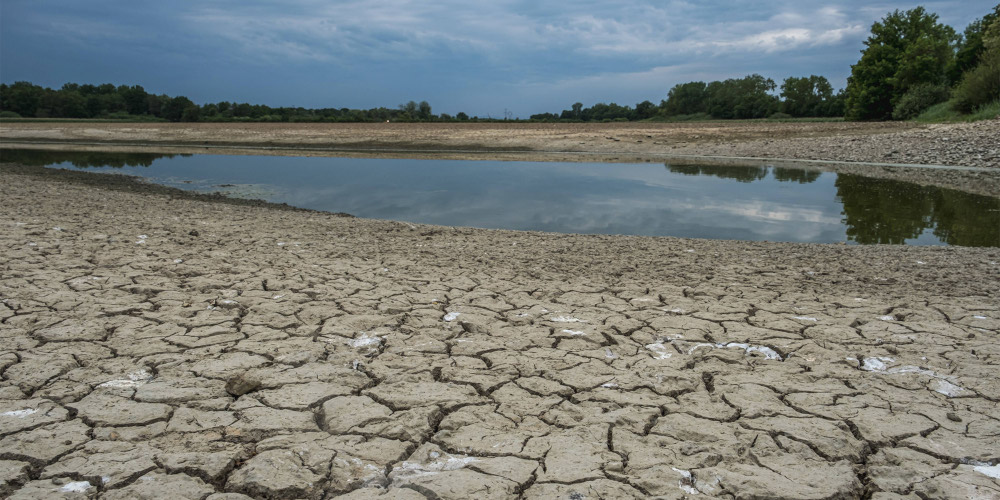
\includegraphics[width=.9\linewidth]{img/secheresse}};
    \node at (0,0) {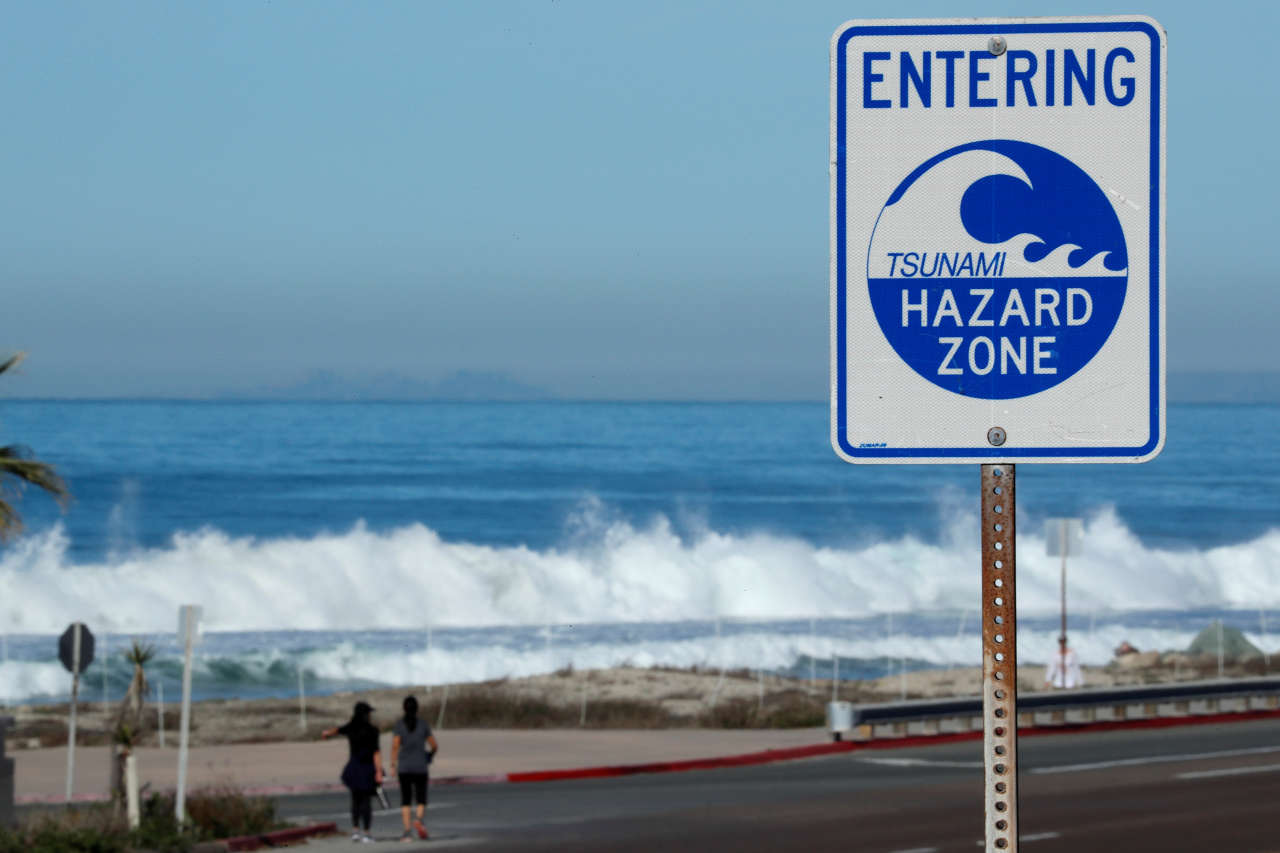
\includegraphics[width=.8\linewidth]{img/tsunami}};
    \end{tikzpicture}        
    \end{figure}
\end{minipage}




}}

{\frame{
\frametitle{Les accords de Paris}

\begin{minipage}{0.4\linewidth}
\textbf{Accords de Paris}

Engagements des pays à réduire les émissions de gaz à effet de serre par  leurs \og CDN \fg (Contribution déterminée au niveau national).

~\ \\

\textbf{Il y a encore du chemin}

Les CDN actuelles amènent à une augmentation des émissions de GES de 15\% en 2030 par rapport à 2010 là où il faudrait que celles-ci soit réduites de 25\% pour l'objectif de 2°C.

\end{minipage}
\hfill
\begin{minipage}{0.5\linewidth}
\begin{figure}
	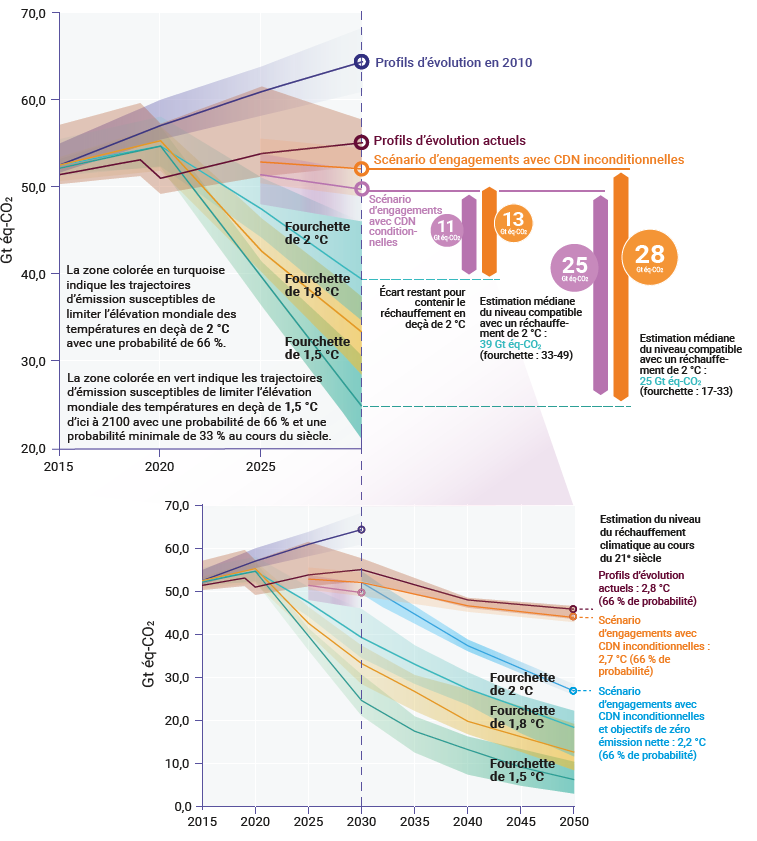
\includegraphics[width=1\linewidth]{img/profils_evolution.png}
\end{figure}
\end{minipage}
}}

{\frame{
\frametitle{Adaptation et atténuation : la lutte contre le changement climatique}

Même limité à +1,5°C, le réchauffement climatique aura un impact important, et qui s'aggravera avec chaque dixième de degré de réchauffement supplémentaire. 

\begin{figure}
	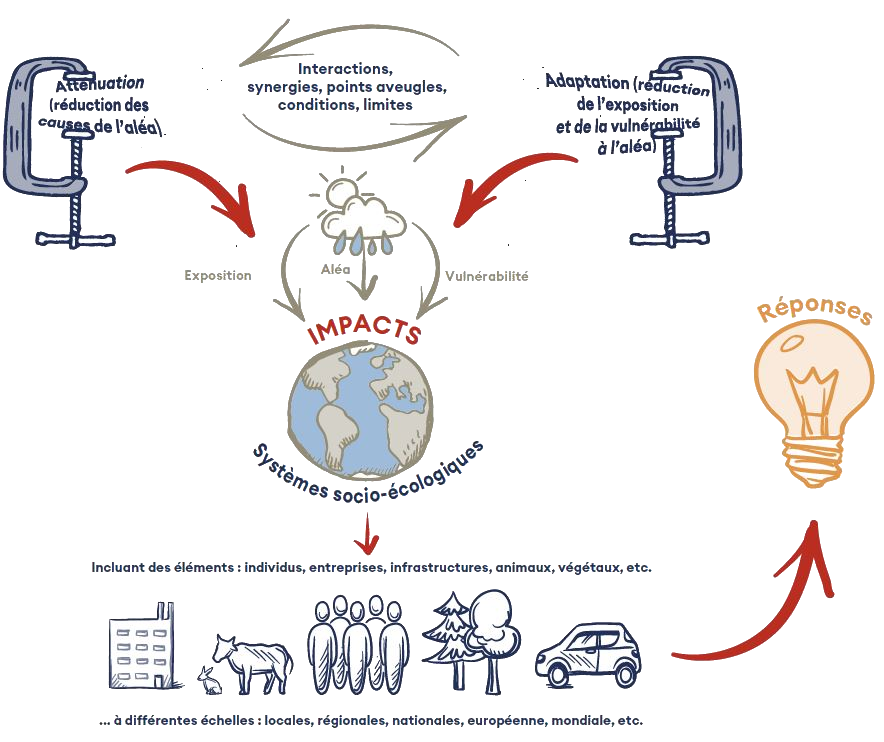
\includegraphics[width=0.6\linewidth]{img/adaptation_attenuation_deux_reponses_0}
\end{figure}
}}




{\frame{
\frametitle{Conclusion}

\textit{70\% des élèves-ingénieurs considèrent la lutte contre le réchauffement climatique et l’innovation dans les nouvelles sources d’énergie comme l’enjeu majeur aujourd’hui.} (09/2020 Ausy, filiale en ingénierie du groupe Randstad)

Dans les prochaines années, les ingénieurs vont avoir un grand rôle à jouer dans la lutte contre le réchauffement climatique et les défis à relever sont immenses:
\begin{itemize}
 \item essayer de rendre la société plus sobre sans trop baisser le niveau de vie,
 \item se passer des énergies fossiles,
 \item revoir la mobilité des personnes,
 \item diminuer les déchets/augmenter le recyclage,
 \item ...
\end{itemize}

\begin{tiny}
Sources:
\vspace{-0.2cm}
\begin{itemize}
 \item \url{https://www.statistiques.developpement-durable.gouv.fr/sites/default/files/2022-04/datalab_essentiel_275_bilan_energetique_provisoire_2021_avril2022.pdf}
 \item \url{https://archivephase1.concertation-strategie-energie-climat.gouv.fr/comprendre/pourquoi-strategie-francaise-lenergie-climat}
\end{itemize}
\end{tiny}

}}

\end{document}

